% ============================================================================
% Capítulo 4 — Desenvolvimento da solução Web
% ============================================================================
\section{DESENVOLVIMENTO DA SOLUÇÃO WEB}

\subsection{Visão geral}

A aplicação Web foi construída em ASP.NET Core 10, com o padrão
Model-View-Controller (MVC) para as telas administrativas e uma camada de API
REST versionada para o consumo pelo aplicativo mobile e por integrações futuras.
A mesma solução hospeda as duas superfícies: o navegador recebe páginas
renderizadas no servidor, enquanto o aplicativo consome JSON sob o prefixo
\texttt{/api/v1}. Essa decisão reduz o custo operacional de manter dois
artefatos e garante que regras de negócio sejam aplicadas uma única vez.

A interface utiliza Bootstrap 5 com identidade visual própria, baseada em tons de
verde, tipografia legível e formulários com validação no cliente e no servidor.
Todas as páginas compartilham um layout com menu lateral, área de conteúdo
principal, mensagens de retorno e link de acessibilidade para saltar diretamente
ao conteúdo.

\subsection{Arquitetura e organização}

O projeto Web é dividido em controladores MVC, controladores de API, view models,
visões Razor e serviços de apresentação. A Tabela~\ref{tab:telas} relaciona as
telas implementadas, a rota de acesso e o público autorizado.

\begin{table}[H]
  \centering
  \caption{Telas da aplicação Web}
  \label{tab:telas}
  \fontsize{9}{11}\selectfont
  \begin{tabular}{L{3.4cm}L{3.6cm}L{5.4cm}L{2.2cm}}
    \toprule
    \textbf{Tela} & \textbf{Rota} & \textbf{Função} & \textbf{Perfil} \\
    \midrule
    Login & \texttt{/Account/Login} & Autenticação por cookie & Público \\
    Painel & \texttt{/} & Indicadores e atalhos & Todos \\
    Produtores & \texttt{/Produtores} & Cadastro e aprovação & Admin \\
    Cooperativas & \texttt{/Cooperativas} & Cadastro de cooperativas & Admin \\
    Produtos & \texttt{/ProdutosWeb} & Catálogo e preços & Admin \\
    Pedidos & \texttt{/PedidosWeb} & Lista, detalhe e status & Admin, Comprador \\
    Entregas e rotas & \texttt{/EntregasWeb} & Rotas, entregas e nova rota & Admin, Motorista \\
    Faturas & \texttt{/Faturas} & Emissão e consulta & Admin \\
    Relatórios & \texttt{/Relatorios/}\allowbreak\texttt{VendasPorProdutor} & Vendas por produtor & Admin \\
    Inclusão & \texttt{/Inclusao} & Produtores por comunidade & Admin \\
    Usuários & \texttt{/Usuarios} & Contas e papéis & Admin \\
    Auditoria & \texttt{/Usuarios/Auditoria} & Trilha de ações & Admin \\
    Privacidade & \texttt{/Home/Privacidade} & Política de dados & Público \\
    \bottomrule
  \end{tabular}

  \vspace{2pt}
  {\fontsize{10}{12}\selectfont\itshape Fonte: elaborado pelo autor (2026)}
\end{table}

A Figura~\ref{fig:painel} apresenta o painel principal, que reúne indicadores de
produtores ativos, pedidos em aberto, entregas pendentes e faturamento do
período, além de atalhos para as operações mais frequentes.

\begin{figure}[H]
  \centering
  \caption{Painel principal da aplicação Web}
  \label{fig:painel}
  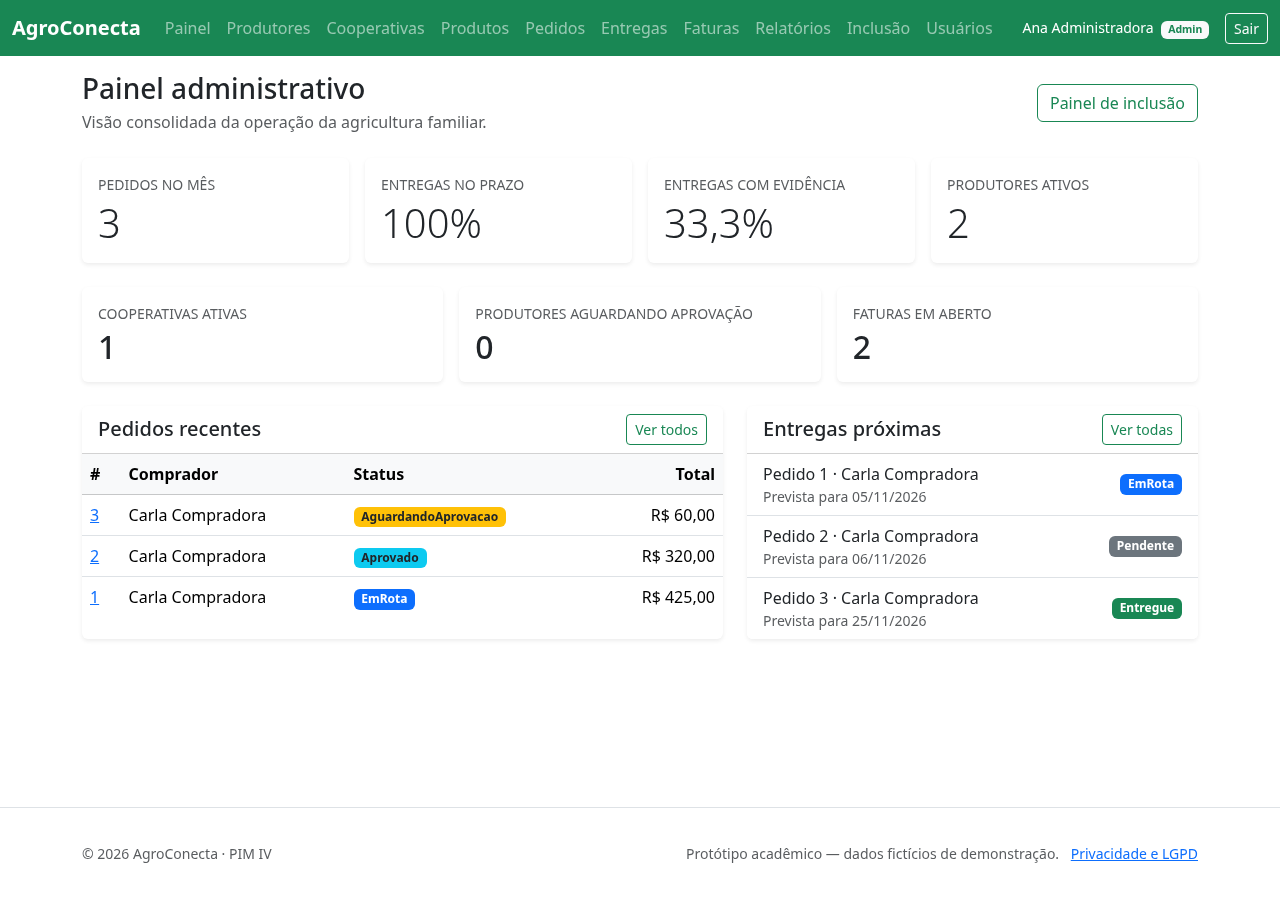
\includegraphics[width=0.80\textwidth]{figuras/painel.png}
  \fonte{elaborado pelo autor (2026)}
\end{figure}

\subsection{Autenticação e controle de acesso}

A autenticação Web utiliza cookie seguro emitido pelo ASP.NET Core Identity,
com proteção antiforgery em todos os formulários POST. As políticas de
autorização são declaradas por papel: \texttt{SomenteAdmin},
\texttt{GerenciarCatalogo}, \texttt{Comprar}, \texttt{OperarPedidos} e
\texttt{Entregar}. O escopo dos dados também é verificado: um comprador só
acessa seus próprios pedidos e recebe resposta 404 -- e não 403 -- ao tentar
consultar recurso de terceiros, evitando a exposição da existência do registro.

\subsection{Cadastros e operação}

Os cadastros de produtores, cooperativas e produtos utilizam formulários com
validação declarativa e mensagens em português, com listagens que exibem a
situação do cadastro e a comunidade de origem.

A operação de pedidos concentra o fluxo comercial. A Figura~\ref{fig:pedidos}
apresenta a listagem com filtros por status e o detalhe do pedido, que exibe
itens, lote de origem, endereço de entrega e histórico de status.

\begin{figure}[H]
  \centering
  \caption{Gestão de pedidos}
  \label{fig:pedidos}
  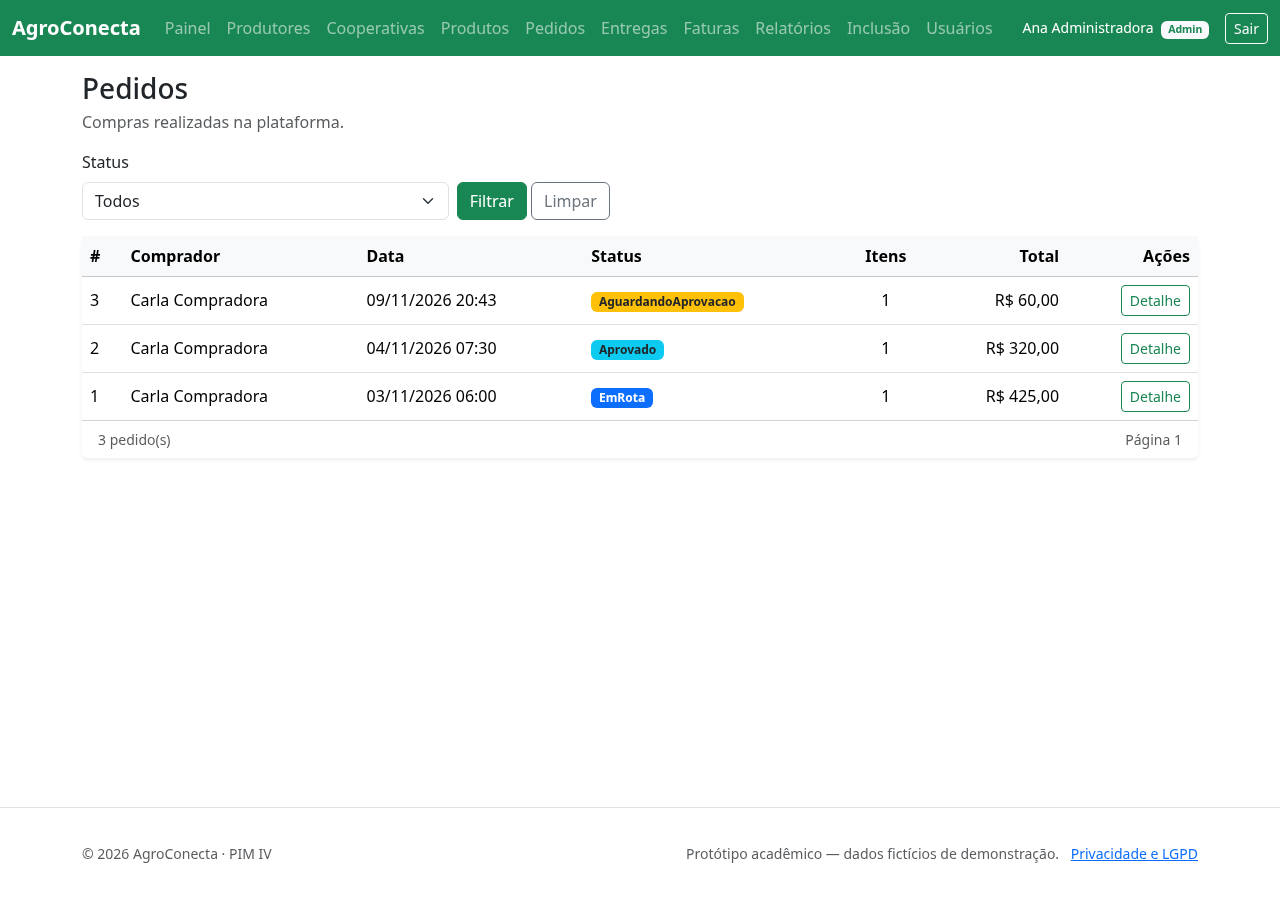
\includegraphics[width=0.80\textwidth]{figuras/pedidos.png}
  \fonte{elaborado pelo autor (2026)}
\end{figure}

As entregas são agrupadas em rotas. Cada rota possui data, motorista, veículo e
um conjunto de pedidos; ao ser criada, gera automaticamente uma entrega por
pedido, conforme a Figura~\ref{fig:entregas}.

\begin{figure}[H]
  \centering
  \caption{Entregas e rotas programadas}
  \label{fig:entregas}
  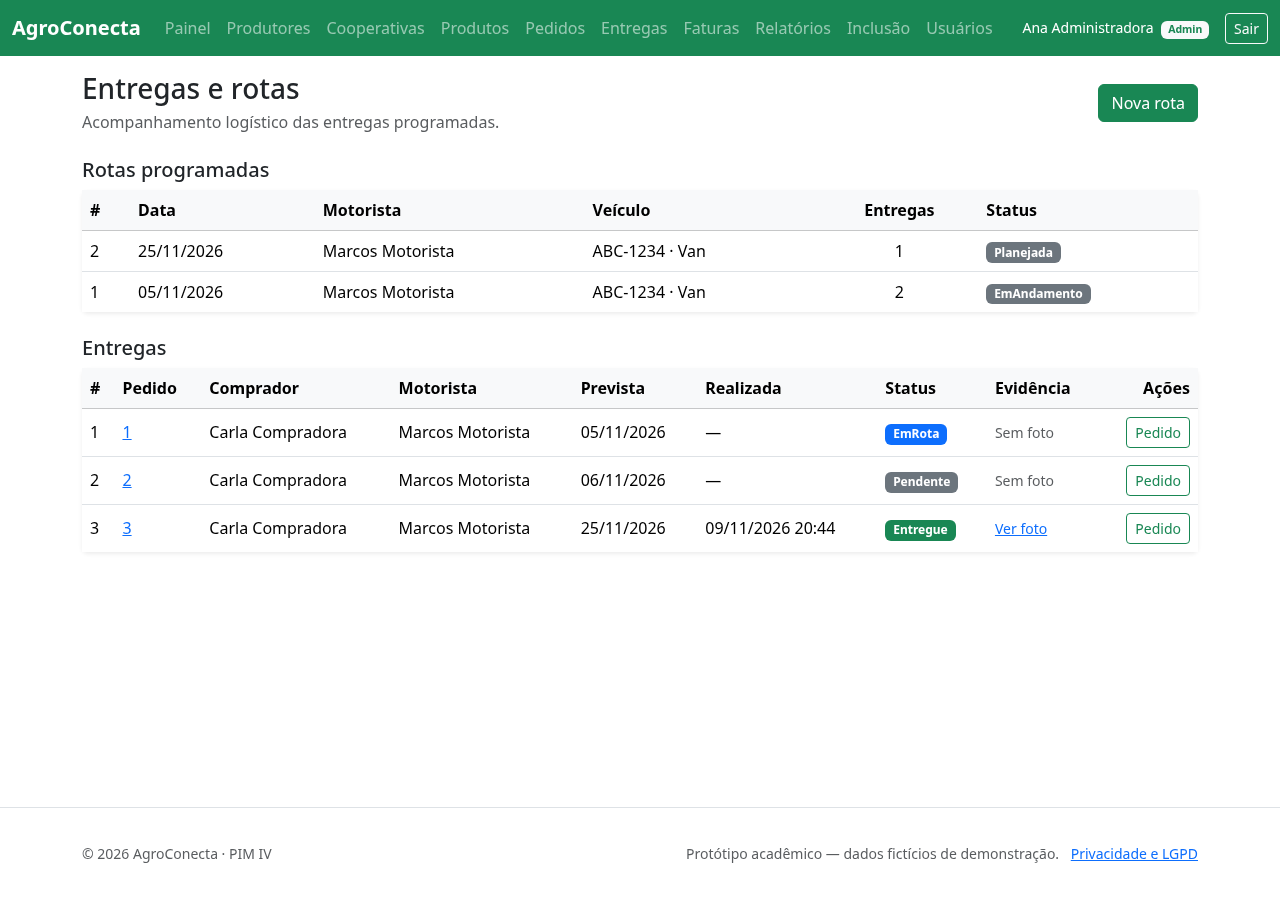
\includegraphics[width=0.80\textwidth]{figuras/entregas.png}
  \fonte{elaborado pelo autor (2026)}
\end{figure}

O faturamento é realizado a partir do pedido, com geração idempotente: se a
fatura já existir, a operação retorna o registro existente em vez de duplicá-lo.
A numeração segue o padrão \texttt{FAT-ANO-SEQUENCIAL}, como ilustrado na
Figura~\ref{fig:faturas}.

\begin{figure}[H]
  \centering
  \caption{Consulta e emissão de faturas}
  \label{fig:faturas}
  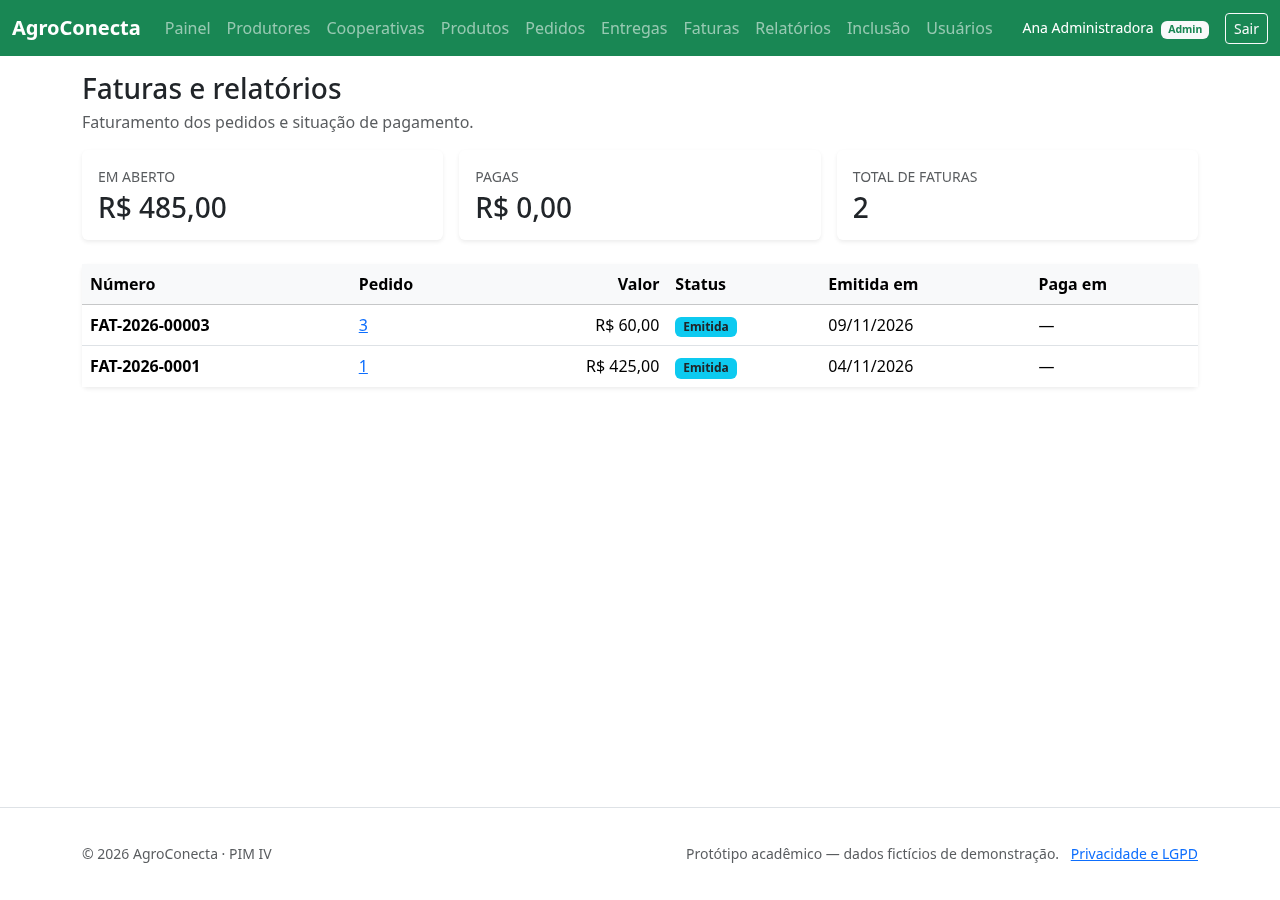
\includegraphics[width=0.80\textwidth]{figuras/faturas.png}
  \fonte{elaborado pelo autor (2026)}
\end{figure}

\subsection{Relatórios e indicadores}

O relatório de vendas por produtor consolida, por período, a quantidade
comercializada e o valor total de cada associado, permitindo comparar
comunidades e orientar políticas de crédito e fomento. A consulta é executada
por procedimento armazenado no banco, o que reduz o tráfego de dados e aproveita
a capacidade de agregação do SGBD. A Figura~\ref{fig:relatorios} apresenta o
resultado com dados de demonstração.

\begin{figure}[H]
  \centering
  \caption{Relatório de vendas por produtor}
  \label{fig:relatorios}
  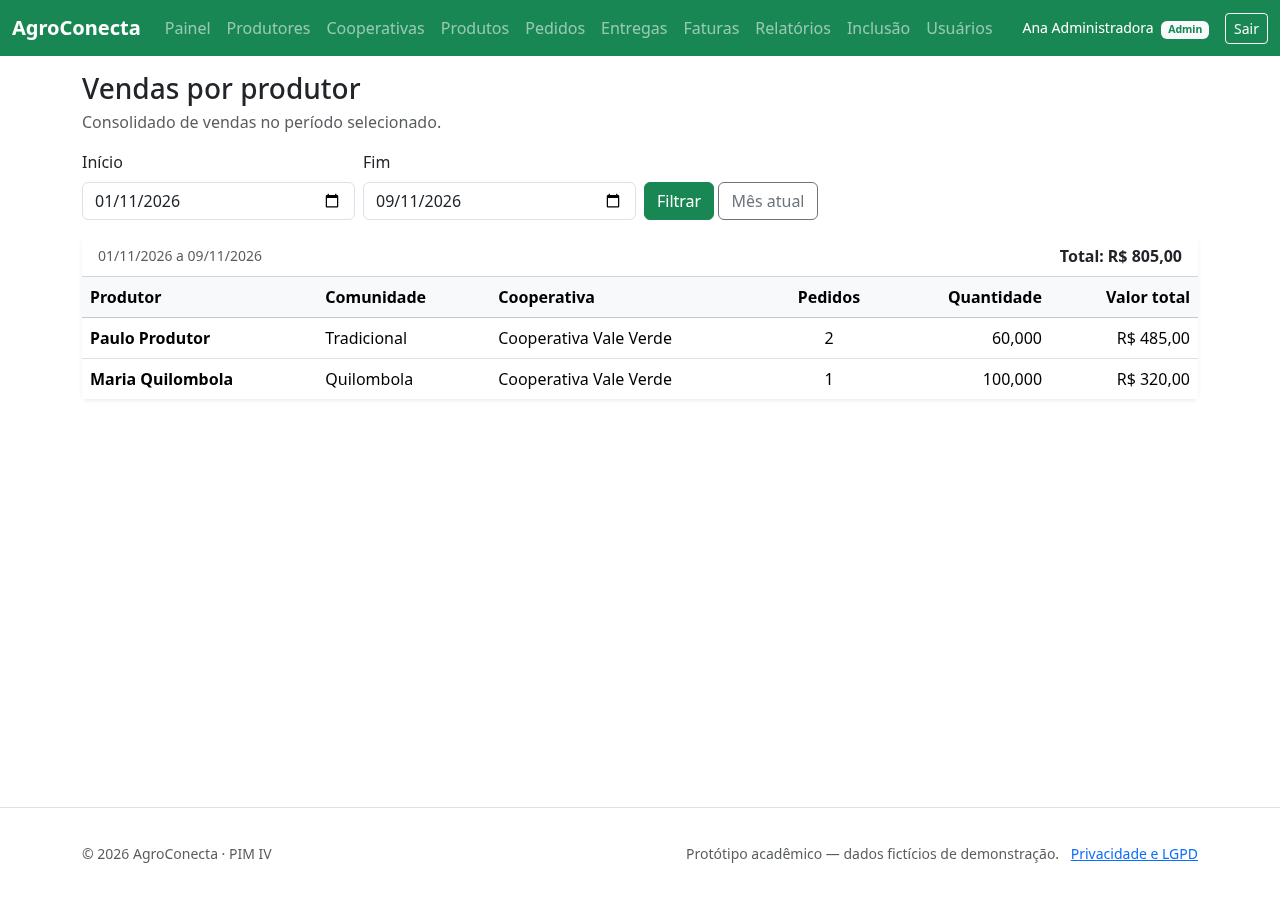
\includegraphics[width=0.80\textwidth]{figuras/relatorios.png}
  \fonte{elaborado pelo autor (2026)}
\end{figure}

Além do relatório, a API expõe um endpoint de indicadores que alimenta o painel
e o aplicativo: número de produtores ativos, pedidos no período, entregas
pendentes, faturamento e percentual de telas acessíveis. Os valores são
calculados no servidor, garantindo consistência entre Web e mobile.

\subsection{API REST e contrato}

A API é versionada em \texttt{/api/v1}, documentada com OpenAPI 3.0 e protegida
por JWT com token de acesso de curta duração e refresh token separado. Os erros
seguem o padrão RFC 7807 (\emph{Problem Details}), com identificador de
correlação para rastreamento. A Tabela~\ref{tab:endpoints} lista os caminhos
publicados.

\begin{table}[H]
  \centering
  \caption{Endpoints da API}
  \label{tab:endpoints}
  \fontsize{9}{11}\selectfont
  \begin{tabular}{L{6.8cm}L{2.2cm}L{6.0cm}}
    \toprule
    \textbf{Caminho} & \textbf{Métodos} & \textbf{Finalidade} \\
    \midrule
    \texttt{/health} & GET & Estado da aplicação \\
    \texttt{/api/v1/auth/login} & POST & Autenticação e emissão de tokens \\
    \texttt{/api/v1/auth/refresh} & POST & Renovação do token de acesso \\
    \texttt{/api/v1/auth/logout} & POST & Encerramento da sessão \\
    \texttt{/api/v1/me} & GET & Perfil do usuário autenticado \\
    \texttt{/api/v1/produtos} & GET, POST & Catálogo \\
    \texttt{/api/v1/produtos/\{id\}} & GET, PUT, DELETE & Manutenção de produto \\
    \texttt{/api/v1/lotes} & GET, POST & Lotes de colheita \\
    \texttt{/api/v1/lotes/meus} & GET & Lotes do produtor autenticado \\
    \texttt{/api/v1/lotes/\{id\}} & GET & Detalhe do lote \\
    \texttt{/api/v1/pedidos} & GET, POST & Pedidos \\
    \texttt{/api/v1/pedidos/\{id\}} & GET & Detalhe do pedido \\
    \texttt{/api/v1/pedidos/\{id\}/status} & PATCH & Transição de status \\
    \texttt{/api/v1/entregas/minhas} & GET & Entregas do motorista \\
    \texttt{/api/v1/entregas/\{id\}/status} & PATCH & Atualização de entrega \\
    \texttt{/api/v1/entregas/\{id\}/evidencia} & PUT & Evidência multipart \\
    \texttt{/api/v1/rotas} & GET, POST & Rotas e geração de entregas \\
    \texttt{/api/v1/faturas} & GET & Consulta de faturas \\
    \texttt{/api/v1/faturas/pedido/\{pedidoId\}} & POST & Emissão idempotente \\
    \texttt{/api/v1/indicadores} & GET & Indicadores do painel \\
    \texttt{/api/v1/relatorios/vendas-produtor} & GET & Relatório por período \\
    \texttt{/api/v1/auditoria} & GET & Trilha de auditoria \\
    \bottomrule
  \end{tabular}

  \vspace{2pt}
  {\fontsize{9}{11}\selectfont\itshape Fonte: elaborado pelo autor (2026)}
\end{table}

O contrato OpenAPI é mantido em \texttt{contracts/} e tratado como fonte de
verdade: alterações são feitas primeiro nele, depois na implementação e, por fim,
na geração dos tipos TypeScript do aplicativo, disciplina que evitou divergências
entre as duas superfícies.
